\documentclass[10pt]{beamer}
\usetheme{Frankfurt}
\usepackage[british,english]{babel}
\usepackage[latin1,utf8x]{inputenc}
\setbeamercovered{transparent}

\title{Classification Techniques for Process Analysis}
\author{Hind Chfouka\inst{1}, Andrea Corradini\inst{1} and Roberto Guanciale\inst{2}}
\institute{\inst{1} Department of Computer Science, University of Pisa, Italy
\and \inst{2} KTH Royal Institute of Technology, Stockholm, Sweden }	
\makeatletter\date{December 6 2013, Turin}\let\Date\@date
\makeatother

\begin{document}
\begin{frame}
\maketitle
\center{
AI meets Business Processes Workshop \\ 
XIII Conference of the Italian Association for Artificial Intelligence}

\end{frame}

\section{Introduction}

\begin{frame}
\frametitle{Context: Process Mining}

\begin{figure}
\includegraphics[width=280pt]{./item/fig1.pdf}
\end{figure}
\end{frame}


\begin{frame}
\frametitle{Focus: Process Analysis}
We focus on: Process Analysis
\begin{figure}
\includegraphics[width=280pt]{./item/fig1Annotated.pdf}
\caption{Process mining}
\end{figure}

\end{frame}

\section{Running example}
\begin{frame}
\frametitle{An example: Sale Business Process}
\begin{figure}
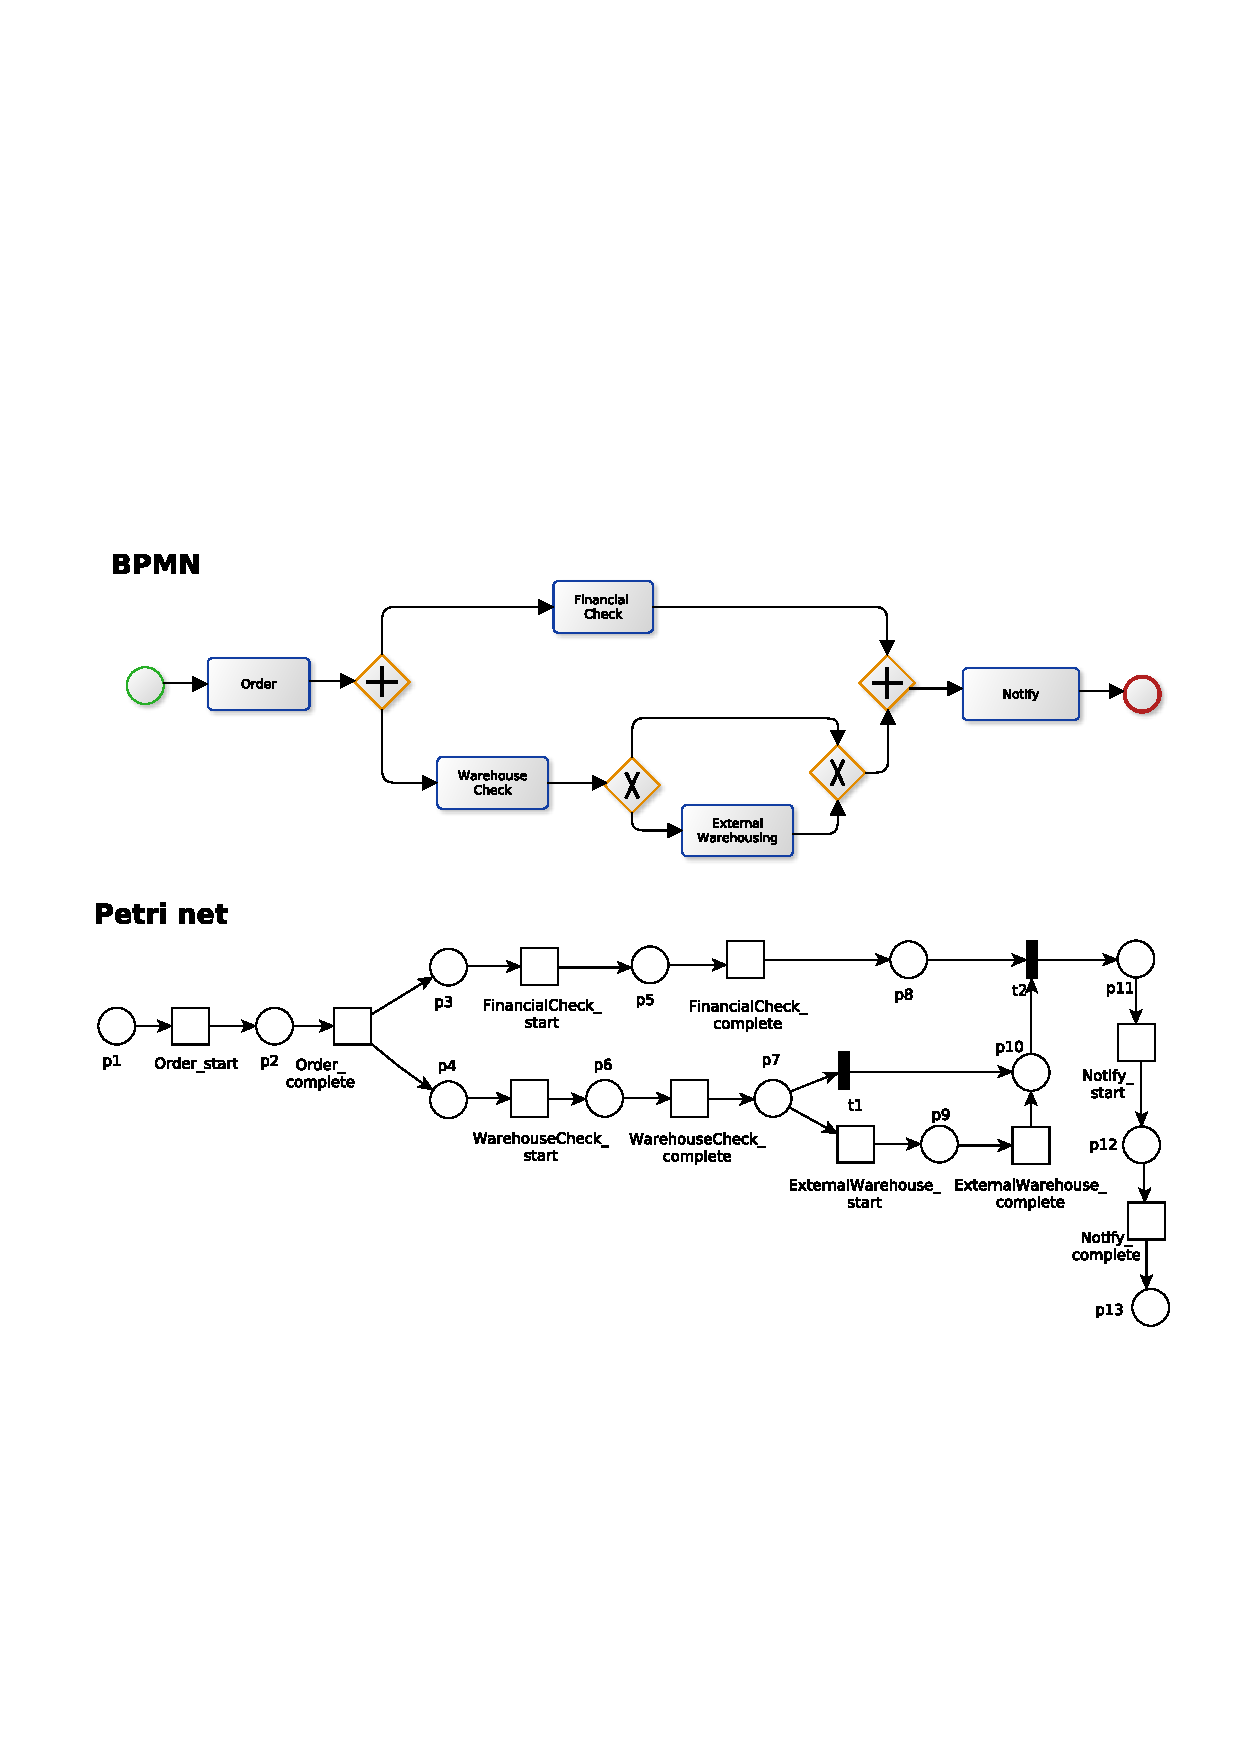
\includegraphics[width=280pt]{./item/SaleProcessModels.pdf}
\caption{Sale Business Process}
\end{figure}
\end{frame}

\section{Process Analysis}
\begin{frame}
\frametitle{ Process Analysis }
\begin{figure}
\includegraphics[width=300pt]{./item/analysis.pdf}
\end{figure}


\end{frame}

\begin{frame}
\frametitle{Log Replay Algorithm}
	\begin{block}{Assumptions}
		\begin{itemize}
		\item Event $e =(a,t,atts)$: the event log building block
		\item Trace: a finite sequence of events $T[1],..., T[n]$ ordered by timestamp. A trace represents a process instance
		\item Event log: a finite sequence of traces
		\item Each event of a trace can be mapped into a transition of the Petri net model
		\end{itemize}
	\end{block}
	\begin{block}{{Algorithm}}
		\begin{itemize}
			\item \alert{Log replay}: executes traces of an event log in a non-blocking way
					\begin{enumerate}
					\item Starts with a token in the start place
					\item Extracts the top event of the log
					\item Fires the corresponding transition in the current marking of the net
						\begin{itemize}
						\item If the transition is not enabled creates the missing tokens artificially
						\end{itemize}
				\end{enumerate}
		\item Log replay results are used in conformance and performance checking
		\end{itemize}
	\end{block}
\end{frame}



\begin{frame}
\frametitle{Conformance Analysis with log replay}
\begin{block}{}
	Conformance checking = check if a trace is compliant with the Petri net model
	\end{block}
	\smallskip
	\smallskip
	\begin{block}{Based on the log replay results...}
		\begin{itemize}
			\item \alert{missing tokens} are generated to mimic an event with a corresponding transition not enabled: this indicates a non-compliance to the model
		\end{itemize}
	\end{block}
\smallskip
\smallskip
\begin{figure}
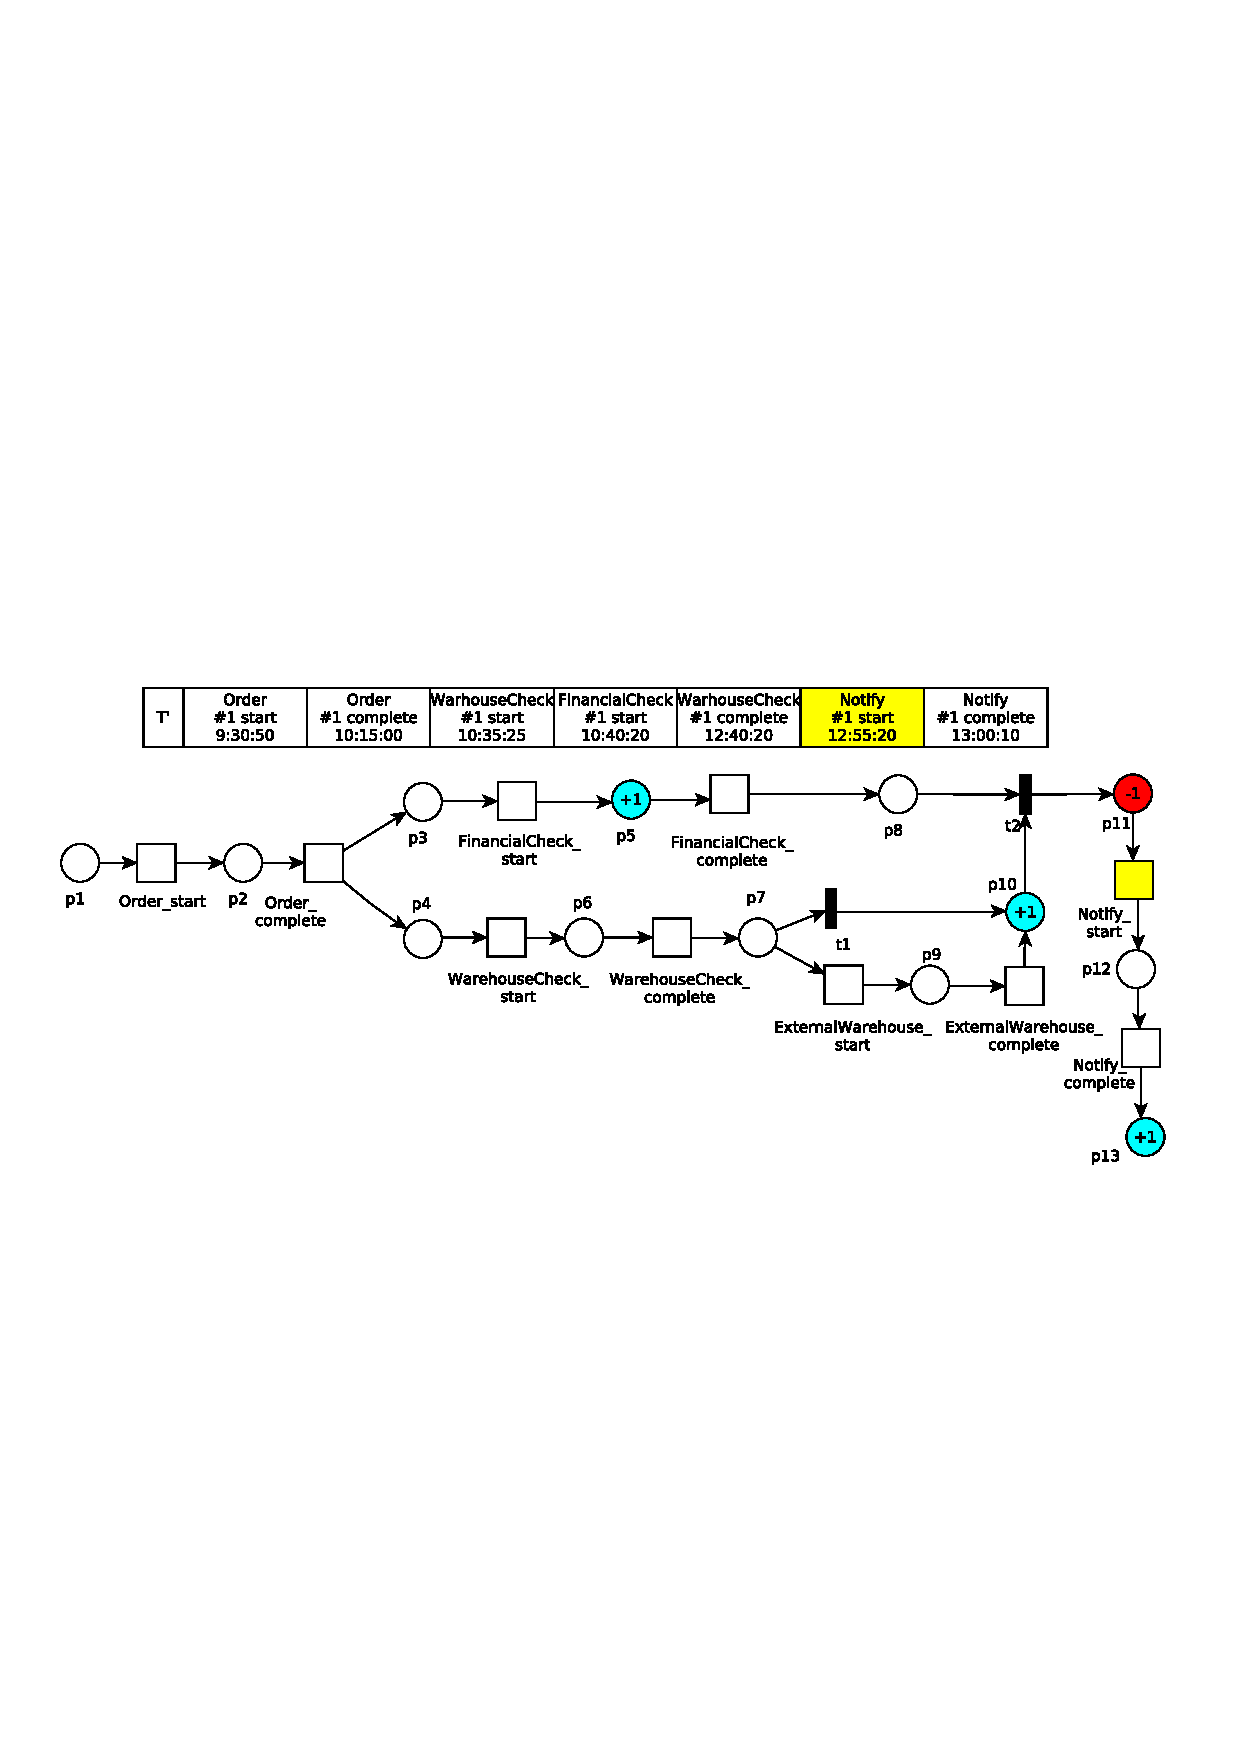
\includegraphics[width=300pt]{./item/conformanceAnalysis.pdf}
\end{figure}
\end{frame}


\section{Machine Learning for Process Analysis}

\begin{frame}
\frametitle{ML for Process Analysis}
\begin{block}{}
Event logs are huge and rich of data: this encourages use of ML techniques\\
\smallskip
Several approaches exploiting Machine Learning techniques for the Business Process understanding:
\begin{itemize}
\item To extract the process model
\item To find rules associated with a decision point
\item To extract implicit information from the data process instances with Data Mining tools
\item ....
\end{itemize} 
\end{block}

\smallskip
\smallskip
\smallskip
\smallskip
\begin{block}{{Our idea}}
Exploiting ML techniques to discover how the {\color{red} process instance data} may influence its {\color{red} conformance}.\\
\end{block}
\end{frame}


\begin{frame}
\frametitle{Classification for Conformance Checking}
Conformance checking problem can be seen as a Classification problem:

\begin{figure}
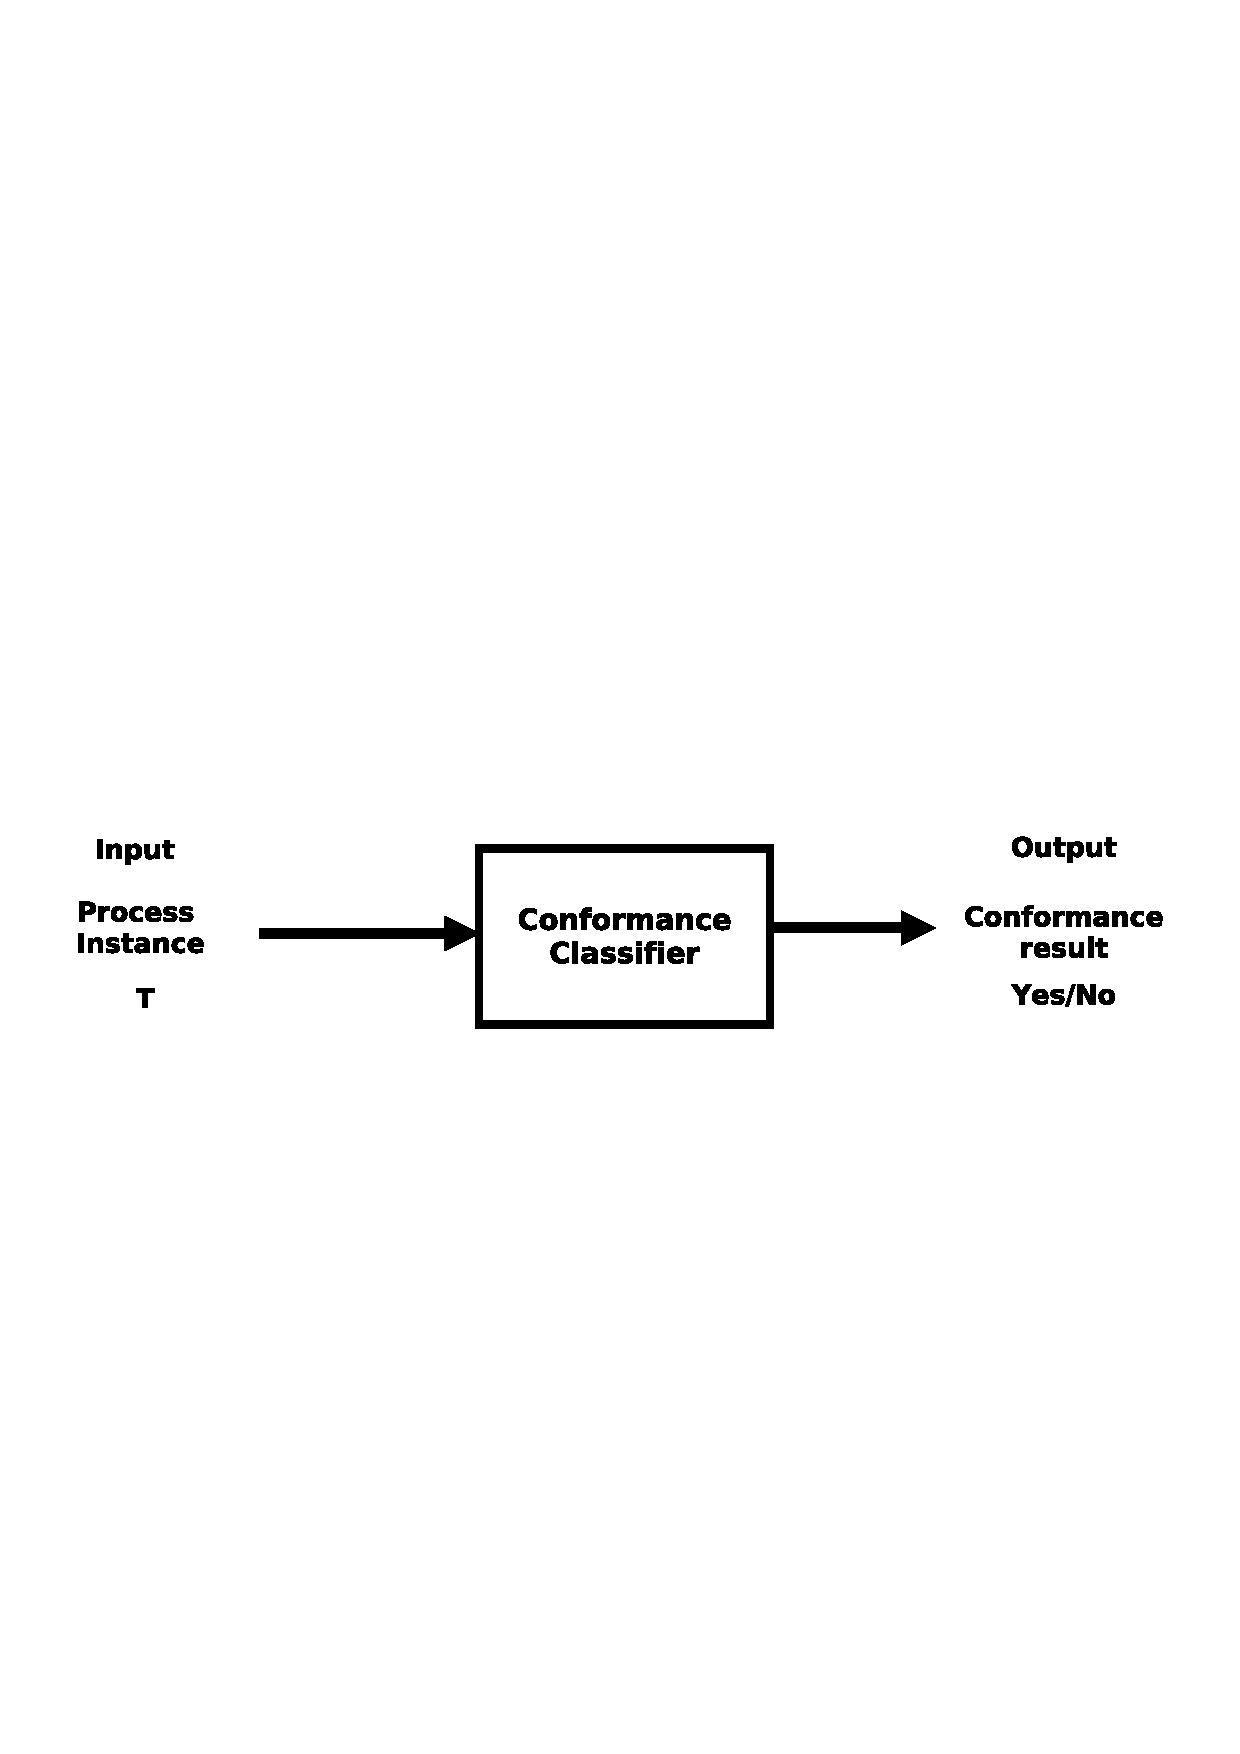
\includegraphics[width=250pt]{./item/classification.pdf}
\end{figure}

Why?
\begin{itemize}
\item To find out patterns of data in correspondence of which conformance errors occur
\item To Predict conformance result at run-time. 
\end{itemize}
How?
\begin{itemize}
\item Learning from previous analysis.
\item Using an explicit classifier: Decision Tree.
\end{itemize}
\end{frame}

\begin{frame}
\frametitle{The approach}
\begin{itemize}
\item {\color{red} Step 1}: collecting a dataset based on event logs
\item {\color{blue} Step 2}: dataset preprocessing including feature selection
\item {\color{green} Step 3}: building a decision tree model using ML algorithm
\item {\color{purple}Step 4}: using the classifier to predict conformance result
\end{itemize}
\smallskip
\smallskip\smallskip
\begin{figure}
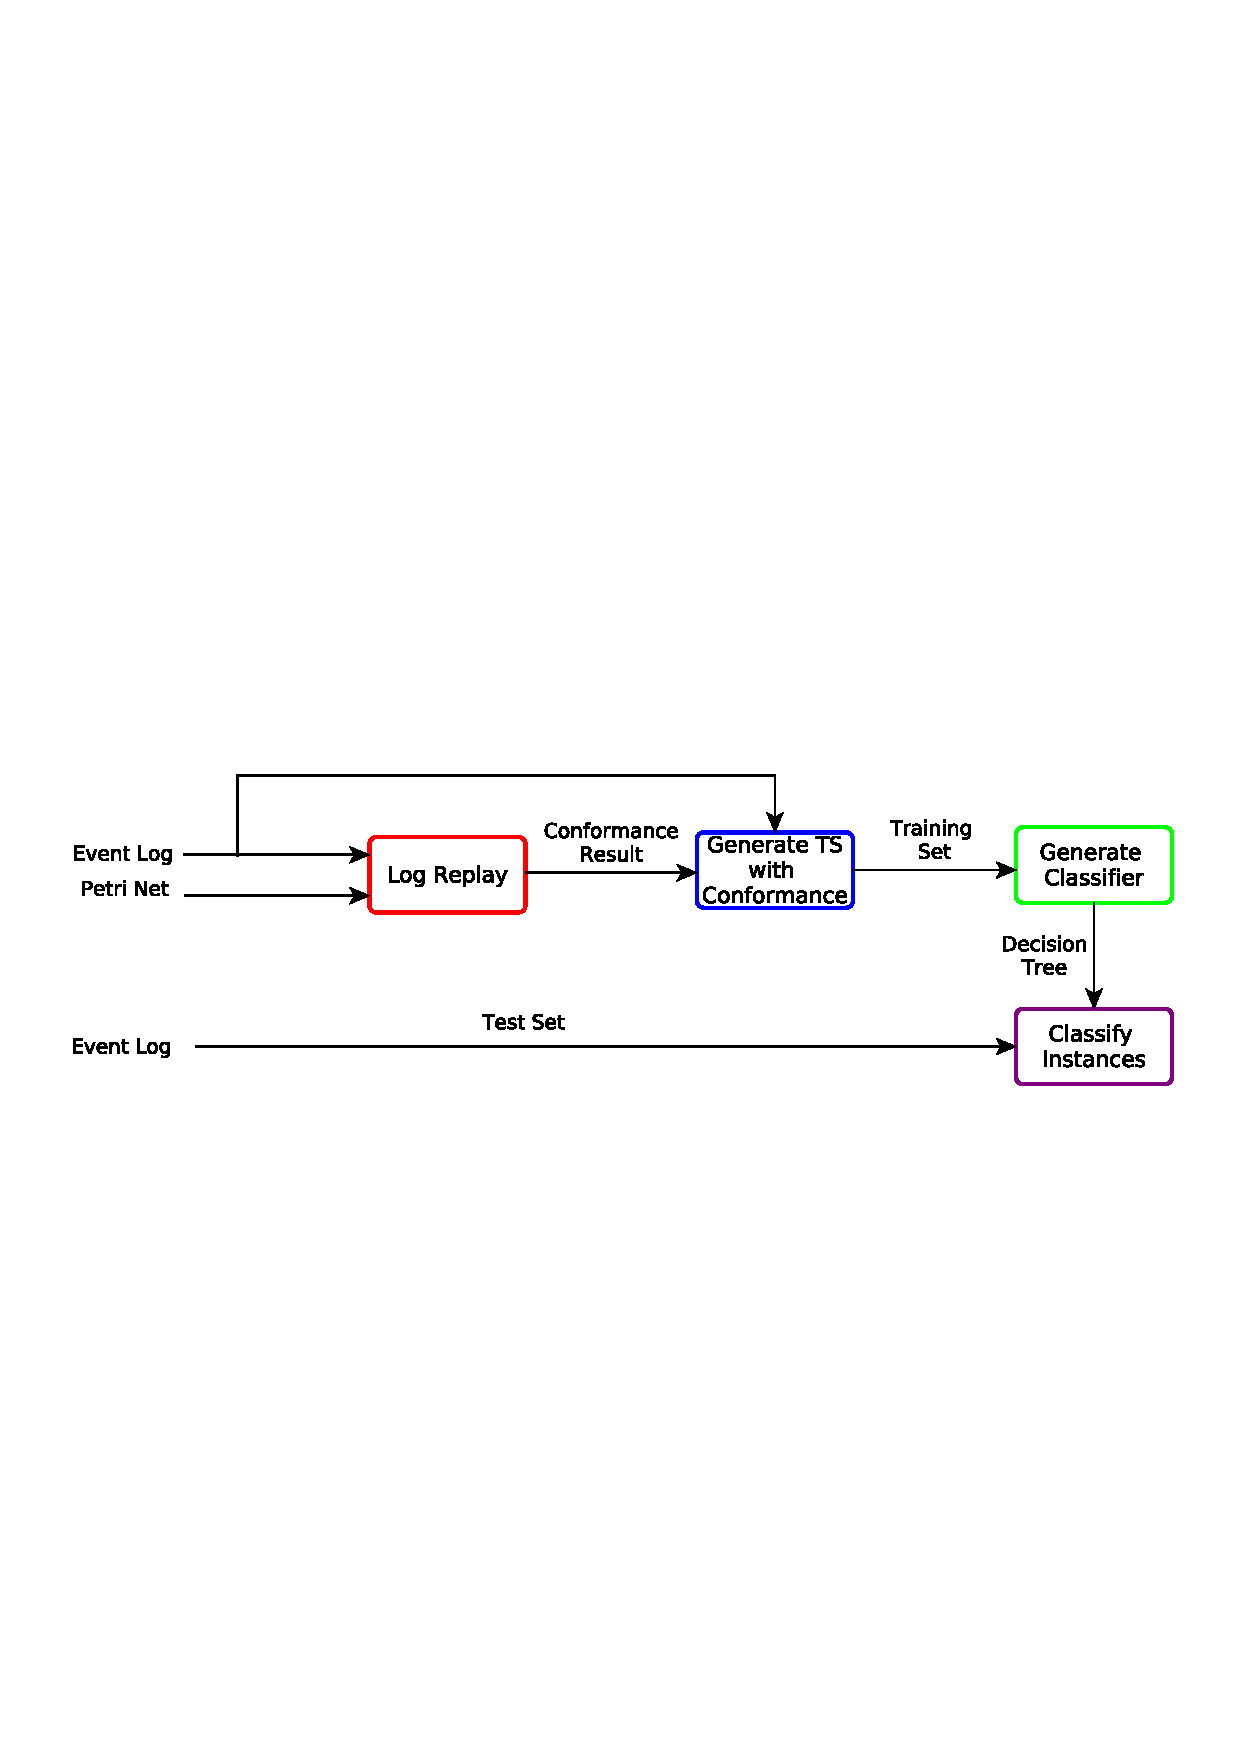
\includegraphics[width=300pt]{./item/methodology.pdf}
\end{figure}
\end{frame}

\begin{frame}
\frametitle{Example: classification for the sale process}
A Petri net summarizing the results of the log replay execution on an event log $L$:
\begin{figure}
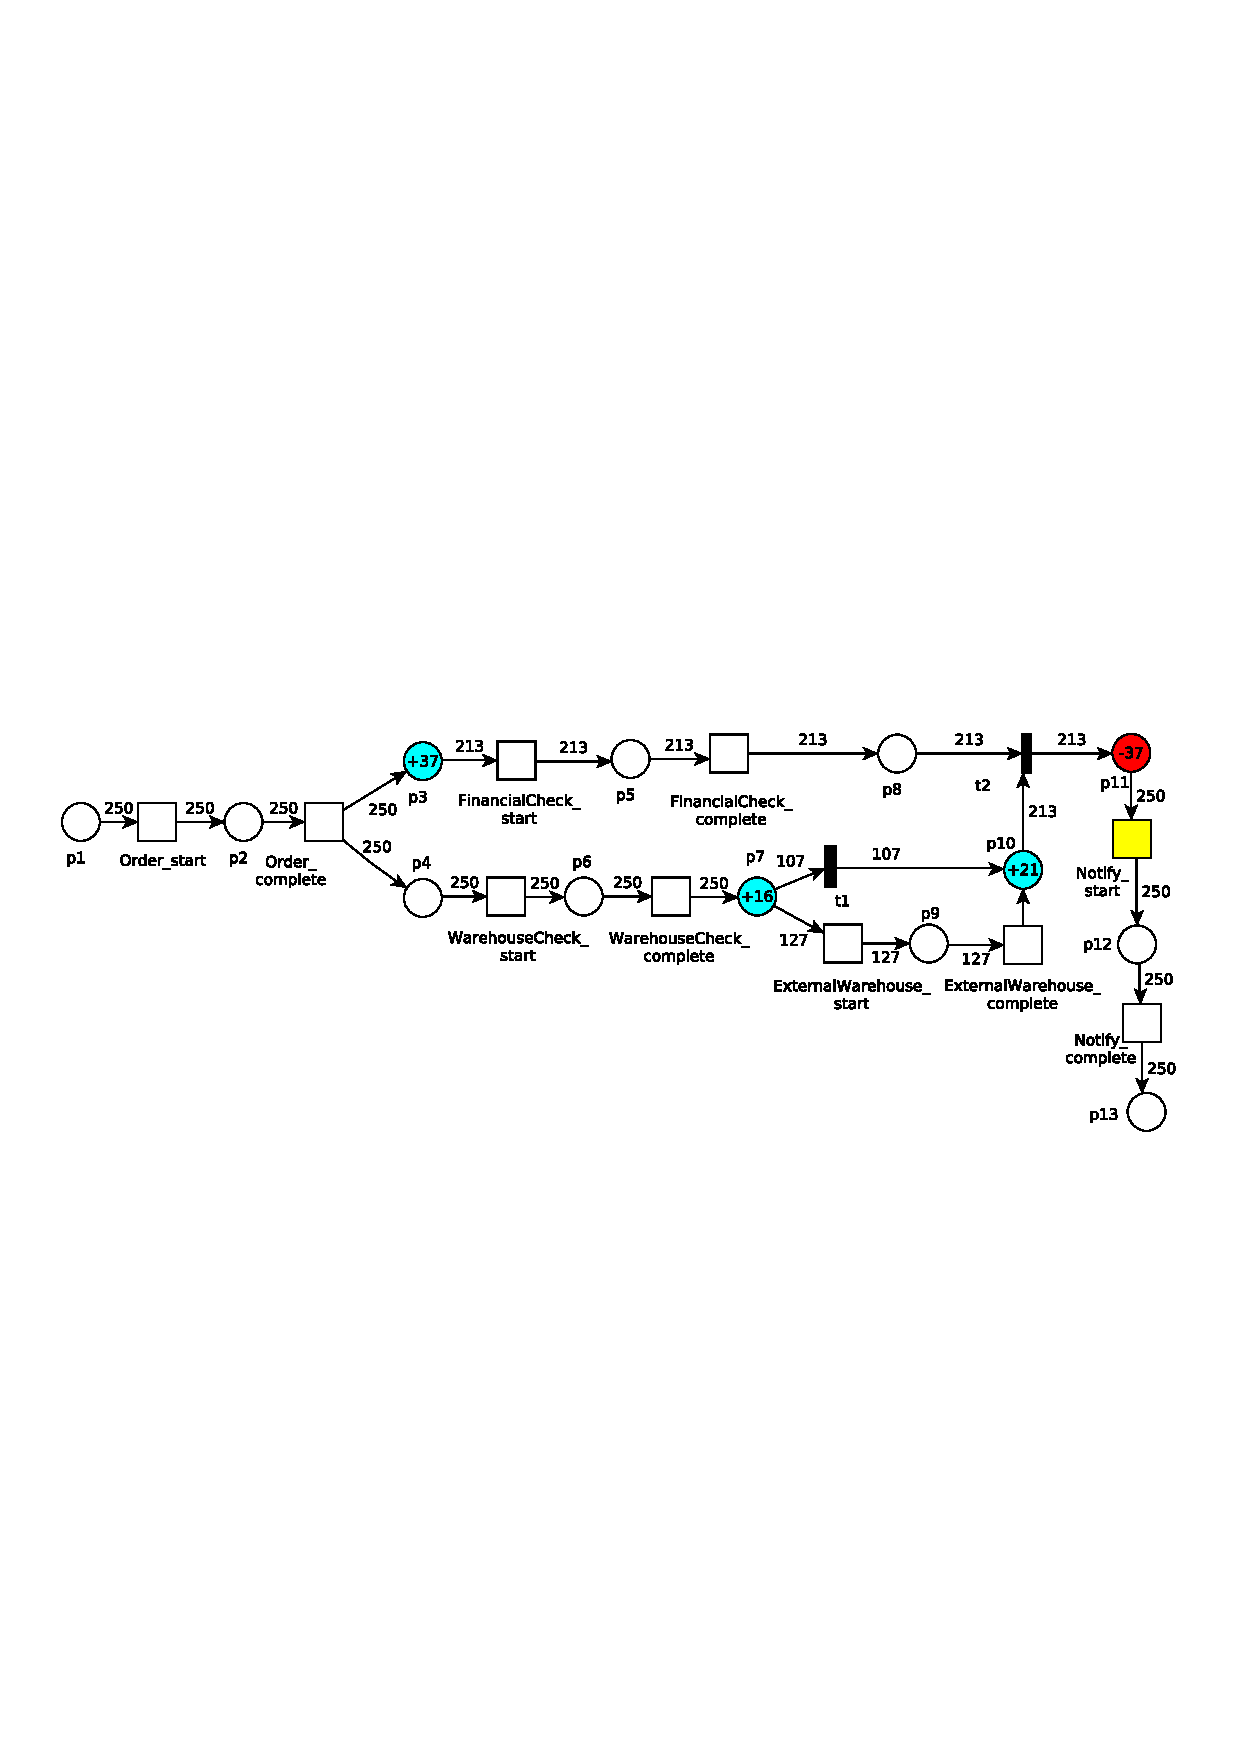
\includegraphics[width=280pt]{./item/Sales_PN_resultMod.pdf}
\end{figure}
37 instances of the process are not compliant with the sale policy since they did not execute the financial check
activity.
\end{frame}

\begin{frame}
\frametitle{Example: classification for the sale process (cont.)}
Log replay conformance results and process data extracted from the event log $L$ enable:
\begin{itemize}
\item the construction of a dataset.
\item the mining of a decision tree.
\end{itemize}
\begin{figure}
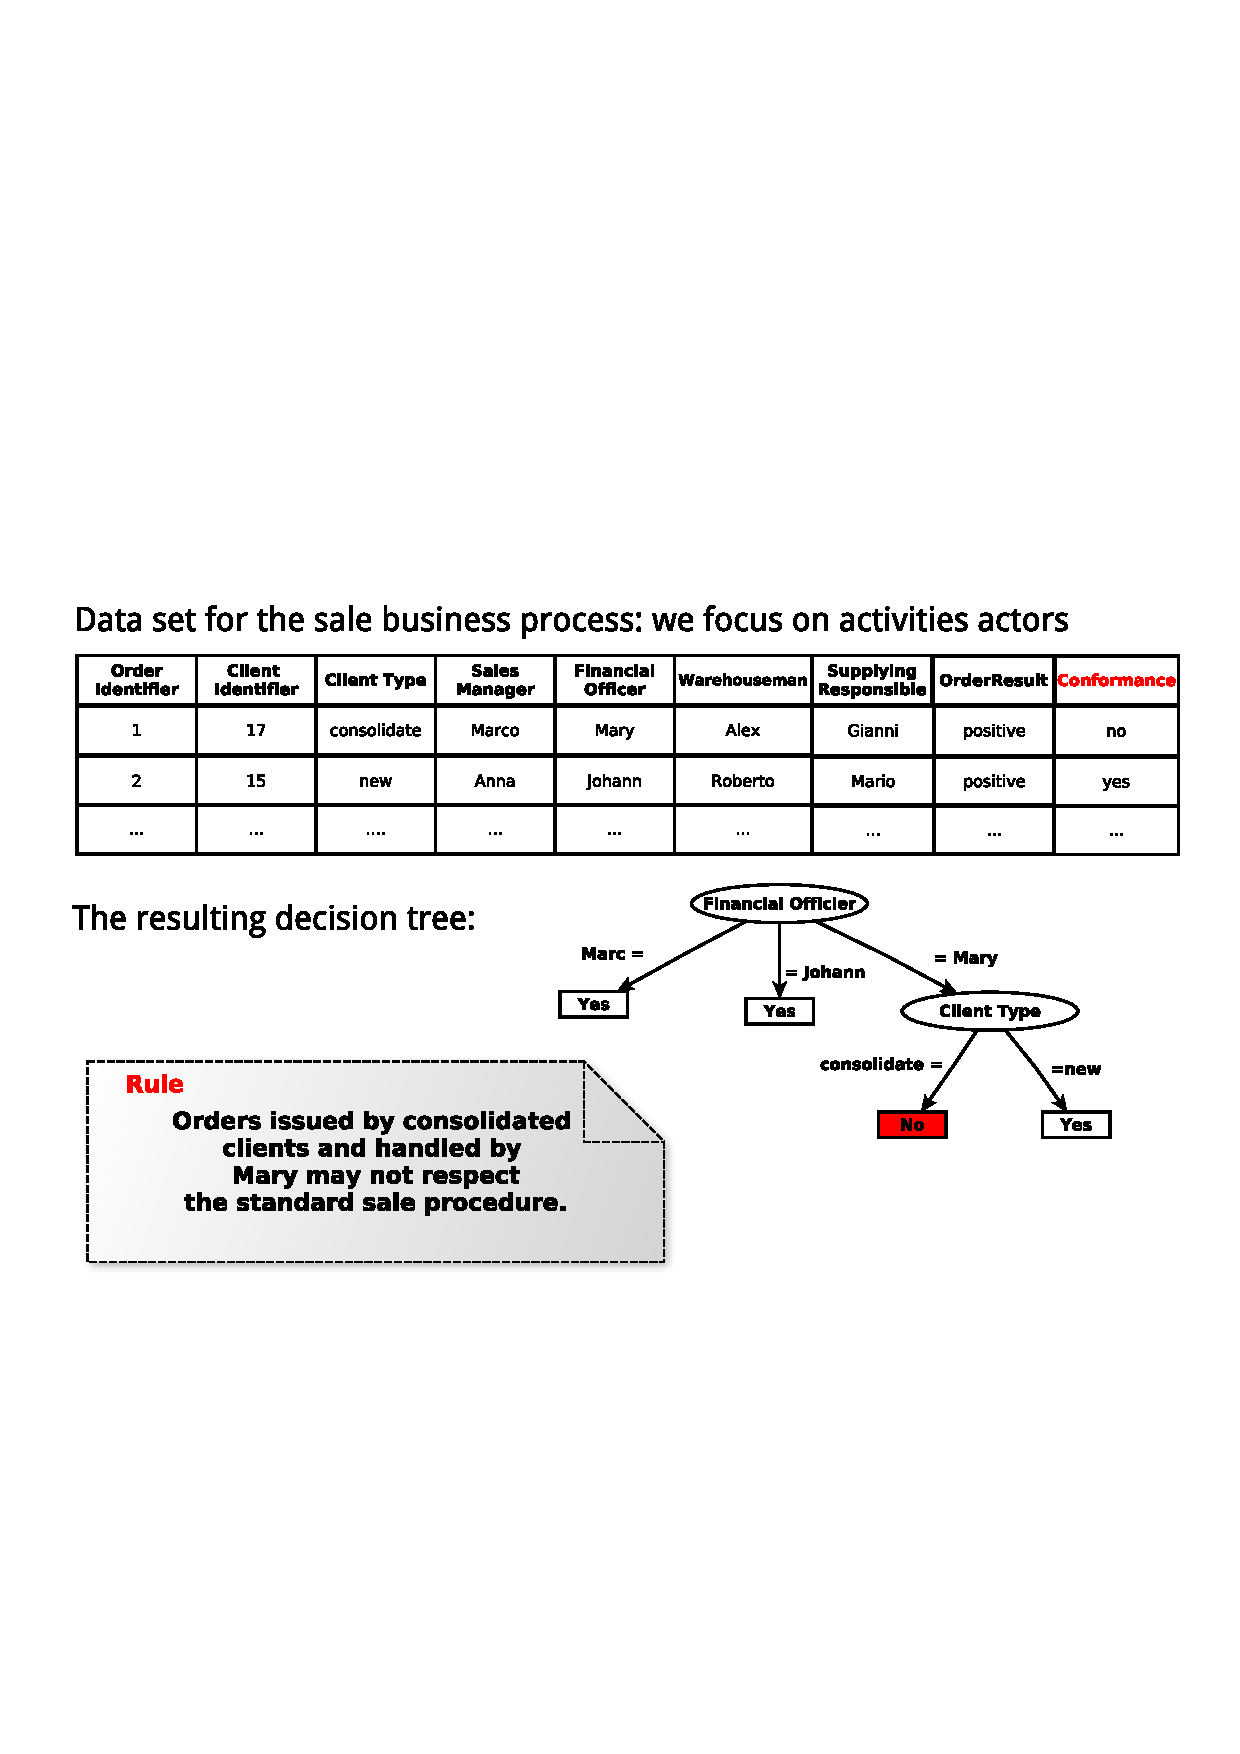
\includegraphics[width=290pt]{./item/casestudy.pdf}
\end{figure}

%Orders issued by consolidated clients and handled by a particular financial officer may not respects the standard sale procedure.
\end{frame}

\section{Framework for the analysis}
\begin{frame}
\frametitle{Framework ProM6}
\begin{figure}
\includegraphics[width=150pt]{./item/prom.pdf}
\end{figure}
\begin{block}{ProM}
\begin{itemize}
\item ProM is an extensible framework that supports a large variety of process mining and analysis techniques.
\item It is a modular software implemented in Java and distributed under GNU Public License (GPL).
\item ProM is a project of Process Mining Group of Eindhoven Technical University, Netherlands.
\end{itemize}
\end{block}
\end{frame}

\begin{frame}
\frametitle{Framework for the analysis}
\begin{figure}
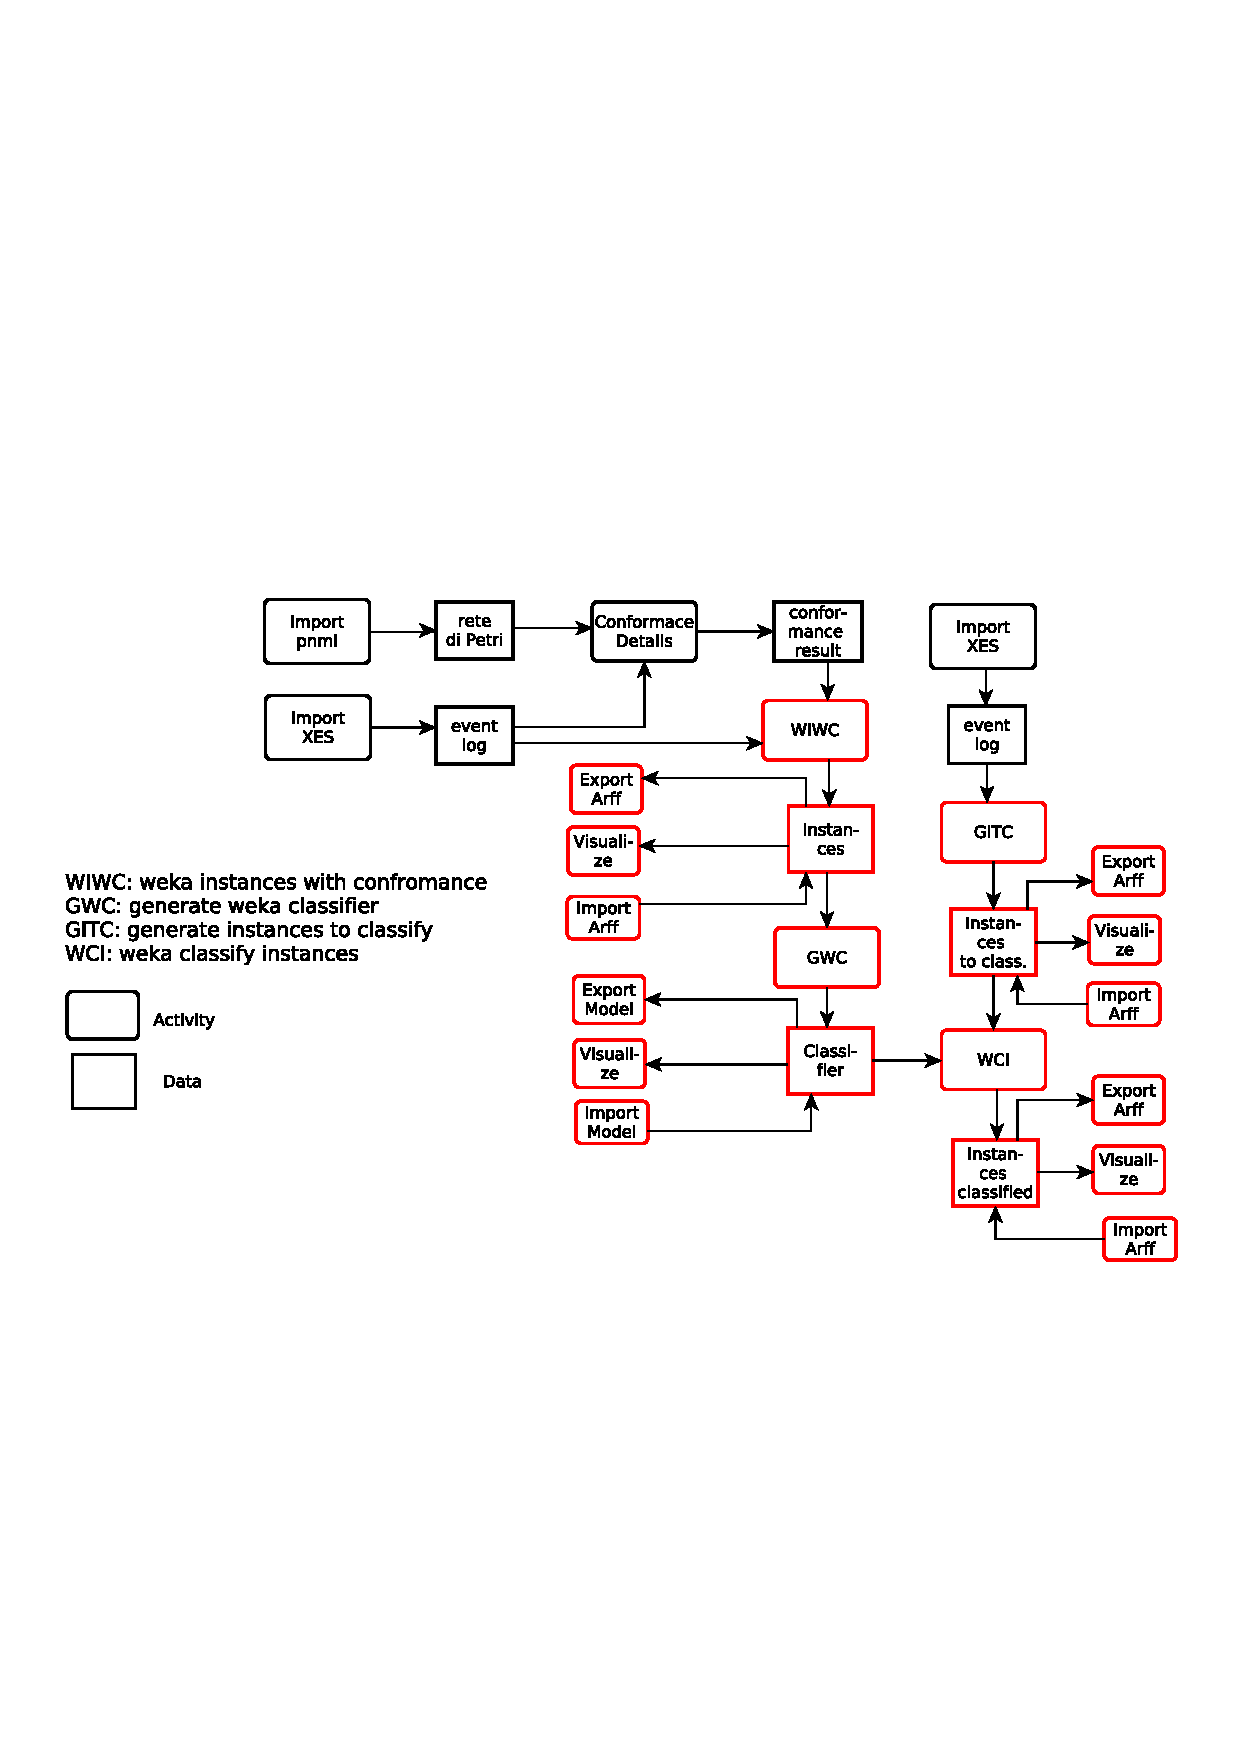
\includegraphics[width=300pt]{./item/worklow.pdf}
\end{figure}
\end{frame}


\section{Conclusion and future works}
\begin{frame}
\frametitle{Conclusion and future works}
Conclusions:
\begin{itemize}
\item Preliminary research aimed at applying ML techniques in the Process Analysis.
\item Extension to performance checking.
\item Experimentation done only with synthetic data.
\end{itemize}
\smallskip
\smallskip
\smallskip
Future Work:
\begin{itemize}
\item Experimentations with real events logs.
\item Exploration of a new technique of conformance checking based on event log alignment.
\end{itemize}

\end{frame}


\end{document}


\begin{comment}
\begin{frame}
\frametitle{Classification Technique}

Few words about the well known machine learning task: classification
\end{frame}
\end{comment}

\begin{frame}


\begin{frame}
\frametitle{Classification for Performance Analysis: an extension}

the approach could be extended to performance analysis:\\
- each join gateway identifies a classification problem
- metrics to be considered as target can be: synchronization time supposing a previous discretization step.

\end{frame}



